\chapter{Realizações}\label{chp:realizacoes}

Durante os estudos de transformações de rotação e translação de objetos em espaço \(\mathbb{R}_3\), o desenvolvimento do projeto fundamentou-se em outros métodos além das disciplinas de Geometria Analítica e Álgebra Linear. Nesse estudo, foram definidas a rotação por ângulos de Euler e a rotação de Rodrigues:

\section{Ângulos de Euler}

É um dos meios de descrever a orientação de um corpo rígido que Leonard Euler formulou.

\section{Parâmetros de Rodrigues}




\section{Calibração}\label{chp:calibr}

O processo de calibração do \textit{VCranium} foi complexo por abranger diversos conceitos de visão computacional e sua aplicabilidade na plataforma do \textit{Unity} \cite{UnityOficial}. Decidimos fragmentar o problema e estudá-los separadamente:

\begin{description}
    \item[Rotação:] Realizado com o \textit{RVEC} de \textit{Rodrigues} de cada \textit{frame};
    \item[Translação:] Realizado com o \textit{TVEC} de \textit{Rodrigues} de cada \textit{frame};
    \item[\textit{Field of View}:] (\textit{FOV}) Calculado com as informações intrínsecas da calibração da câmera;
    \item[Distorção:] Calculado com as informações de distorção da calibração da câmera;
\end{description}

\subsection{Rotação}

A informação da rotação do modelo virtual do cérebro é adquirida da comunicação \textit{socket} com o servidor em \textit{Python}. Abaixo está estruturada o formato da mensagem enviada a cada iteração do computador para a aplicação:

\begin{figure}[ht]
    \centering
    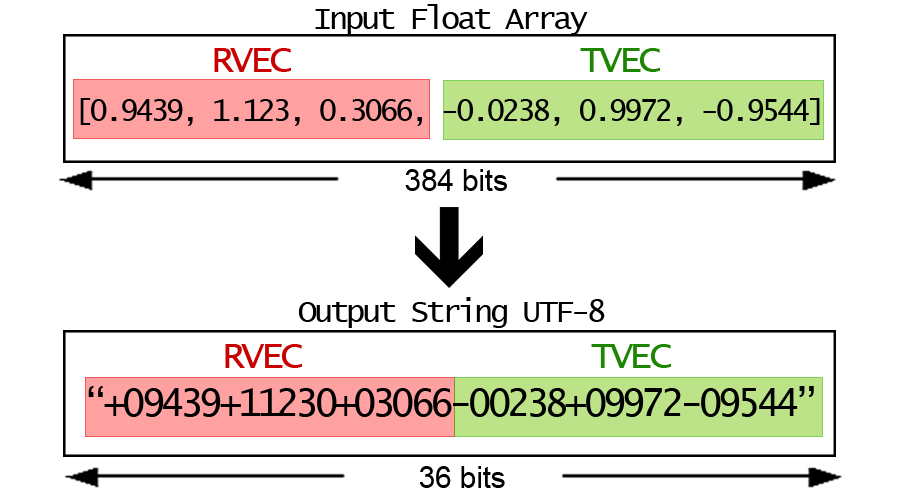
\includegraphics[width=.55\textwidth]{figuras/format rodrigues.png}
    \caption{Estrutura da mensagem via \textit{socket}. Fonte: Autor.}
    \label{fig:frodrigues}
\end{figure}

Um método foi implementado para a formatar cada mensagem gerada pela detecção da posição do marcador, transformando uma lista do \textit{Python} em uma \textit{string} com o formato de \textit{UTF-8}, como é mostrado no \textit{RVEC} da Figura \ref{fig:frodrigues}. Assim que a aplicação recebe os três números, eles representam o vetor de rotação com as coordenadas X, Y e Z, respectivamente. Para descobrirmos a magnitude da rotação neste eixo, deve-se calcular o módulo desse vetor de rotação, o resultado é dado em radianos.

\subsection{Translação}

Da mesma forma que a rotação, a translação é recebida do \textit{TVEC} da mensagem da Figura \ref{fig:frodrigues}. Nesta, a informação é recebida em milímetros, portanto, devemos ajustar a escala da translação manualmente para corrigir a projeção do marcador no mundo virtual do \textit{Unity}. Com a rotação e translação completas, temos a calibração extrínseca da projeção. Assim como foi explicado no último relatório, a projeção deve estar visualmente boa, especialmente nas regiões centrais da tela, representado na Figura \ref{fig:Extrinsecos}.

\begin{figure}[ht]
    \centering
    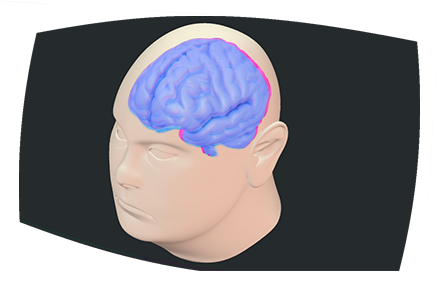
\includegraphics[width=.45\linewidth]{figuras/CalibExtr.png}
    \caption{Exemplo de sobreposição sem calibração intrínseca. Fonte: Autor.}
    \label{fig:Extrinsecos}
\end{figure}

\subsection{\textit{Field of View}}

O \textit{Field of View} (\textit{FOV}) é calculado da calibração da câmera com o \textit{chessboard} que calcula a distorção e os intrínsecos da câmera, nomeados respectivamente de \textit{DIST} e \textit{MTX}. Para determinar o \textit{FOV} da câmera observamos a matriz \textit{MTX} [FONTE]:

\begin{figure}[ht]
    \centering
    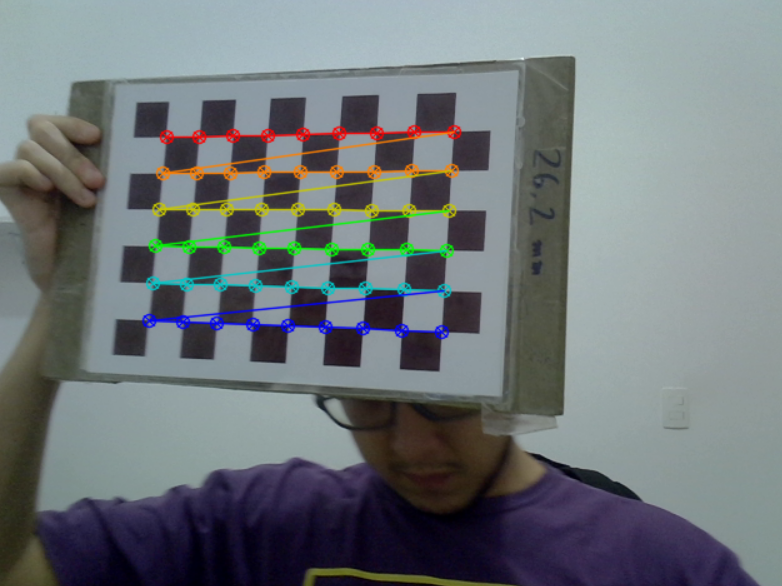
\includegraphics[width=.45\linewidth]{figuras/chessboard.png}
    \caption{Calibração dos intrínsecos da câmera com o \textit{chessboard}. Fonte: Autor.}
    \label{fig:chess_calib}
\end{figure}

\[ MTX = 
\renewcommand\arraystretch{.8}
\begin{bmatrix}
    f_x & 0 & c_x \\
    0 & f_y & c_y \\
    0 & 0 & 1
\end{bmatrix} \]

% DESCREVER PARAMETROS Sendo \(f_x\) o foco em X da câmera e
Utilizamos as distâncias focais da câmera, \(f_x\) ou \(f_y\), e a informação das dimensões da imagem em \textit{pixels} para obter o \textit{FOV} em X e Y: 

\[
FOV_x = 2 \arctan \left( \dfrac{w}{2f_x} \right) ;
\ \ \ FOV_y = 2 \arctan \left( \dfrac{h}{2f_y} \right) 
\]
    
Sendo \(w\) e \(h\) a largura e a altura em \textit{pixels}, respectivamente. Não existe diferença em utilizar qualquer um dos dois, pois o \textit{Unity} suporta ambas as configurações no objeto da câmera virtual.
    
\subsection{Distorção}

% https://en.wikipedia.org/wiki/Pinhole_camera
% https://docs.opencv.org/4.x/dc/dbb/tutorial_py_calibrationtutorial_py_calibration.html
% https://en.wikipedia.org/wiki/Distortion_%28optics%29
A documentação do \textit{OpenCV} baseia-se na câmera \textit{pinhole} e modela duas principais distorções: radial e tangencial. 

\begin{description}
    \item[Radial:] A distorção radial é percebida como retas se curvando em relação ao centro. Causada pela fabricação da forma circular das lentes, o que contribui para um maior campo de visão.
\end{description}
\[ x_{distorted} = x(1+k_1 r^2 + k_2 r^4 + k_3 r^6) \]
\[ y_{distorted} = y(1+k_1 r^2 + k_2 r^4 + k_3 r^6) \]
\begin{figure}[H] % https://learnopencv.com/understanding-lens-distortion/
    \centering
    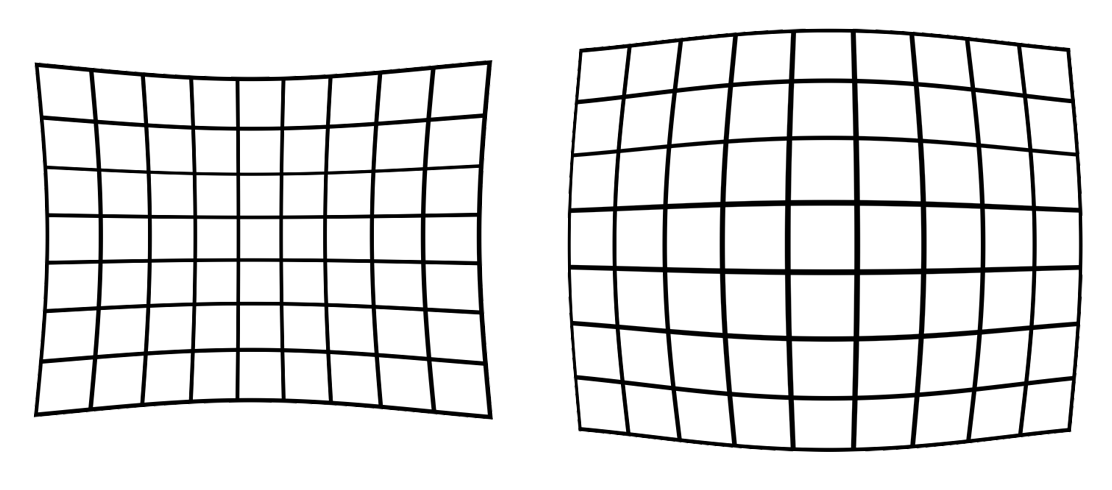
\includegraphics[width=.65\linewidth]{figuras/radial-dist.png}
    \caption{Exemplos de distorção radial. Fonte: Autor.}
    \label{fig:radial_dist}
\end{figure}
\begin{description}
    \item[Tangencial:] A distorção tangencial é percebida em regiões da imagem que parecem mais próximas ou mais distantes da câmera de forma não uniforme. Causada pelas tolerâncias de paralelismo da montagem do sensor com as lentes internas do equipamento.
\end{description}
\[ x_{distorted} = x + 2 p_1 x y + p_2 (r^2 + 2x^2)\]
\[ y_{distorted} = y + p_1(r^2+2y^2)+2p_2xy\]
\begin{figure}[H] 
    \centering
    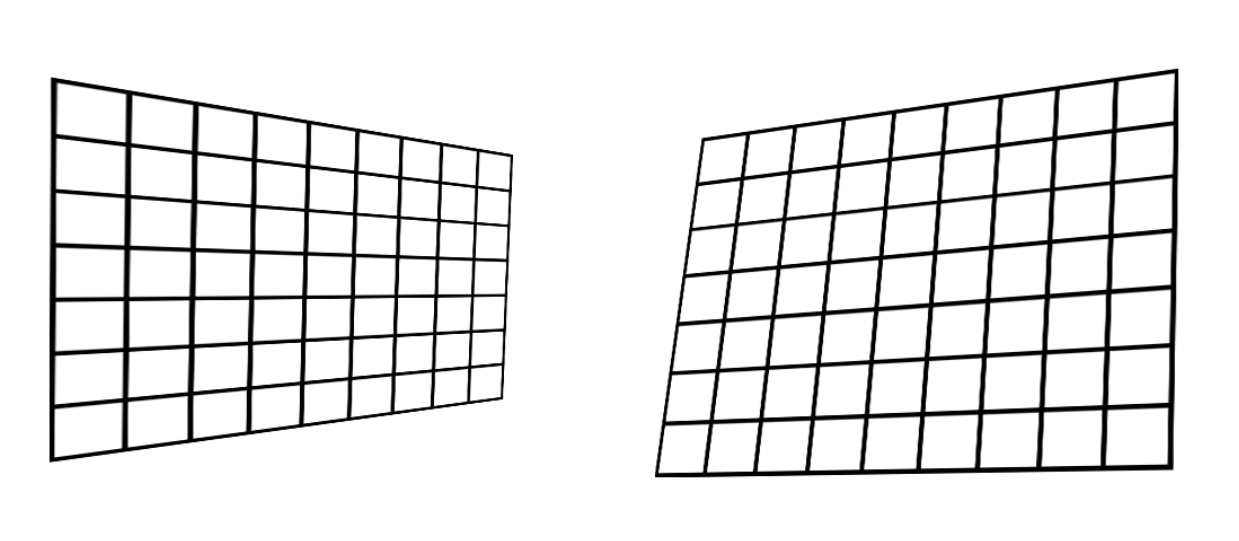
\includegraphics[width=.65\linewidth]{figuras/tan-dist.png}
    \caption{Exemplos de distorção tangencial. Fonte: Autor.}
    \label{fig:tan_dist}
\end{figure}

Utilizando as fórmulas apresentadas acima e os parâmetros intrínsecos \(f_x \ f_y \ c_x \ c_y\) e distorção \(k_1 \ k_2 \ k_3 \ p_1 \ p_2\), tem-se todas as variáveis necessárias para a modelagem da câmera com \textit{OpenCV}:

\[ DIST = [ k_1 \ k_2 \ p_1 \ p_2 \ k_3 ]; \ \ \ \ \ \ \ \
MTX = 
\renewcommand\arraystretch{.8}
\begin{bmatrix}
    f_x & 0 & c_x \\
    0 & f_y & c_y \\
    0 & 0 & 1
\end{bmatrix};\]

\section{Desenvolvimento Unity}

Dada a teoria da visão computacional apresentada na Seção \ref{chp:calibr}, traz-se para a aplicação no ambiente de desenvolvimento \textit{Unity}. Para isso, deve-se organizar de ''cenas'', onde o usuário pode transitar utilizando a interface, como na Figura \ref{fig:ui1}, e utilizar a linguagem C\# como \textit{back-end} para a criação de \textit{scripts}.

\begin{figure}[ht]
    \centering
        \begin{subfigure}{.45\textwidth}
            \centering
            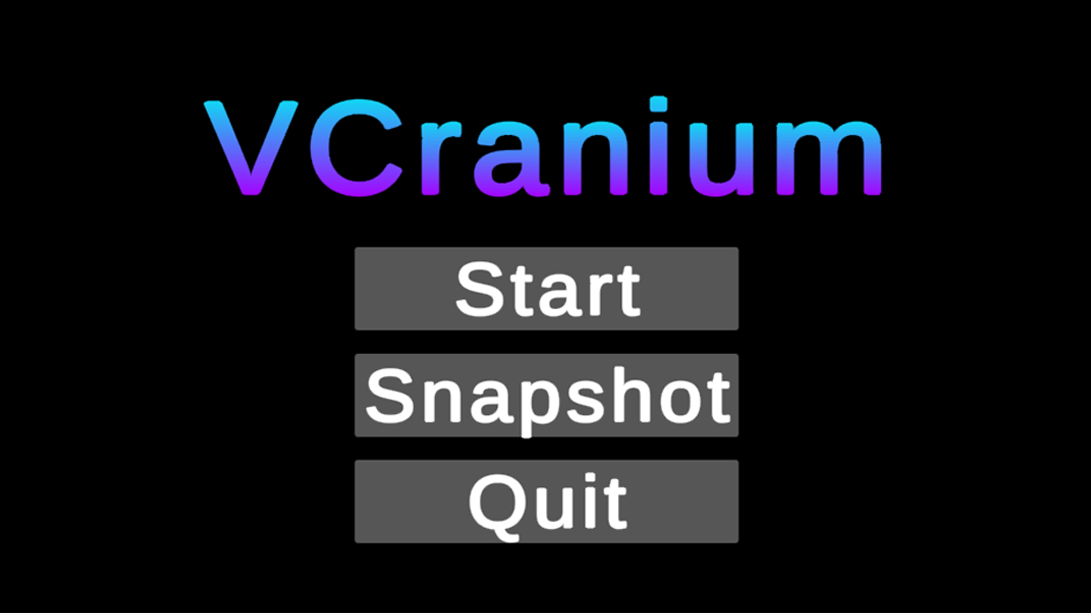
\includegraphics[width=.95\linewidth]{figuras/vcranium_main.png}
            \caption{Menu principal do programa}
            \label{fig:vcranium-connect}
        \end{subfigure}
        \begin{subfigure}{.45\textwidth}
            \centering
            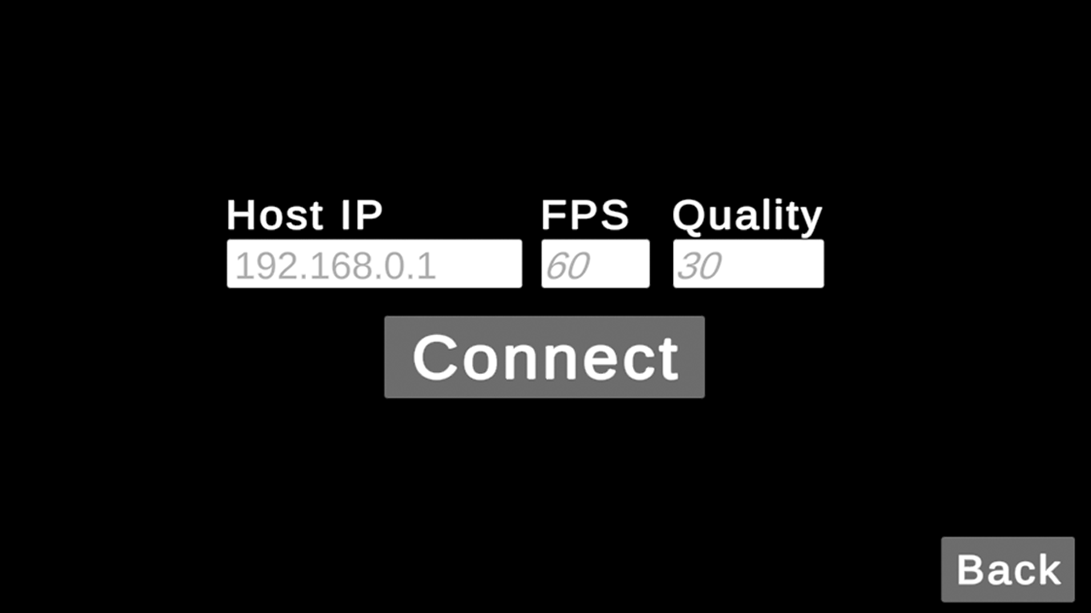
\includegraphics[width=.95\linewidth]{figuras/vcranium_connect.png}
            \caption{Tela de conexão com computador}
            \label{fig:vcranium2-connect}
        \end{subfigure}
        \caption{Imagens da interface do \textit{VCranium}. Fonte: Autor.}
        \label{fig:ui1}
\end{figure}

\subsection{Ajuste dos intrínsecos}

A Seção \ref{chp:calibr} também explicita que obtemos todos os parâmetros intrínsecos e de distorção de uma câmera após a calibração com o método do \textit{chessboard} (Figura \ref{fig:chess_calib}). Porém, é necessário um método que realize a calibração da câmera em que o \textit{VCranium} está sendo executado, para isso, deve-se criar um método auxiliar que capture uma série de imagens e envie para o computador calibrar e encontrar os parâmetros.

A principal ideia que se tem ao criar esse sistema é receber uma imagem assim que o usuário pressionar o botão de captura. Assim como foi estudado em relatórios anteriores, é necessário construir um \textit{header} simples que antecede o envio da imagem para o servidor preparar a sua recepção, e então, guardar a informação de cada imagem em uma lista auxiliar. O próximo passo é usar o comando \textit{calibrateCamera} da biblioteca do \textit{OpenCV} e o programa retorna as informações necessárias (\(f_x, \ f_y, \ c_x, \ c_y, \ k_1, \ k_2, \ k_3, \ p_1, \ p_2\)).

O desenvolvimento desse programa auxiliar não apresenta maiores desafios se comparado com o histórico do projeto desde 2021. No entanto, assim que o aplicativo \textit{Unity} receber todos os parâmetros, não é trivial a distorção do modelo para a sobreposição em uma aplicação de realidade do tipo \textit{VST} (\textit{Video See-Through}).

Visto que seria necessário um estudo mais aprofundado no assunto de calibração, elaboração de conceitos da disciplina de Computação Gráfica para a vista em perspectiva, e a aplicação desse trabalho seriam restritos somente ao modelo \textit{VST}, foi decidido privar a calibração intrínseca do projeto no dado momento. A Figura \ref{fig:Extrinsecos} mostra que ao fim da calibração extrínseca, a sobreposição é visualmente boa, i.e., em boa parte de ilustração, o erro da sobreposição é insignificante e, com isso, não apresenta problemas para demonstração de conceitos.